\documentclass{article}
\usepackage[utf8]{inputenc}
\usepackage{graphicx}
\usepackage{amsmath }
\usepackage{amssymb}
\usepackage{subcaption}
\usepackage{float}
\usepackage{mathtools}
\setcounter{section}{0}


\usepackage{cleveref} %referencing figures, equations and tables
\crefformat{figure}{Figure.~#2#1#3}
\crefformat{equation}{Eq.~#2#1#3}
\crefformat{table}{Table.~#2#1#3}
\crefformat{appendix}{Appendix.~#2#1#3}
\crefformat{section}{Section.~#2#1#3}

\title{L-Shaped Bracket Static Analysis}
\author{Amir Baharvand }
\date{}

\begin{document}

\maketitle

\section{Problem Statement}
The L-shaped bracket, \cref{fig:frame}, is simply supported on the left hole while the lower half-part of the right hole is under a uniform pressure $P = 20$MPa.

\begin{figure}[H]
    \centering
    \includegraphics[width = 0.5\textwidth ]{figures/frame.pdf}
    \caption{The L-shaped bracket geometry, coordinate system and boundary condition.}
    \label{fig:frame}
\end{figure}

\section{Numerical Model}
The problem can be modeled as plane stress because the planes on both sides of the domain in the $z$-direction are stress-free ($\sigma_z = \sigma_{yz} = \sigma_{zx} = 0$) and the thickness is negligible compared to the other geometrical dimensions.

\subsection{Mechanical Properties}
The numerical model unit is set to SI unit in millimeters. \cref{tab:mat_prop_frame} summarizes the mechanical properties of the L-shaped bracket.

\begin{table}[H]
    \centering
    \caption{Mechanical properties of the L-shaped bracket.}
    \begin{tabular}{l c c c} \hline
        Property & Symbol & Unit & Value \\ \hline
        Young's modulus & $E$& MPa & 2E05 \\
        Poisson's ratio & $\nu$ & - & 0.3 \\
        Thickness & $h$ & mm & 5 \\ \hline
    \end{tabular} 
    \label{tab:mat_prop_frame}
\end{table}

\subsection{Solver}
The solver for this problem is set to \textbf{Static, General} because the problem is linear static (no contact, boundary conditions do not change with time). The solver, of course, invokes the Newton-Raphson method. Alternatively, one may use \textbf{Static, Linear perturbation}.

\subsection{Mesh Study}
To achieve a robust numerical model, a mesh convergence study based on the maximum von Mises stress is performed and the relative error w.r.t the former step is calculated from \cref{eq:relative_error}.

\begin{equation}
    \text{Relative error[\%]} = \frac{\sigma_{vm_{\{i+1\}}} - \sigma_{vm_{\{i\}}}}{\sigma_{vm_{\{i+1\}}}} \times 100
    \label{eq:relative_error}
\end{equation}

where $\sigma_{vm}$ is the maximum von Mises stress and $i$ is the step for each level of mesh refinement. \cref{fig:mesh_convergence} shows the mesh convergence plot and based on the relative error values in the last column of \cref{tab:mesh_convergence}, the mesh size 1.25mm is selected for the numerical model. The mesh quality is illustrated in \cref{fig:mesh_quality}.

\begin{figure}[H]
    \centering
    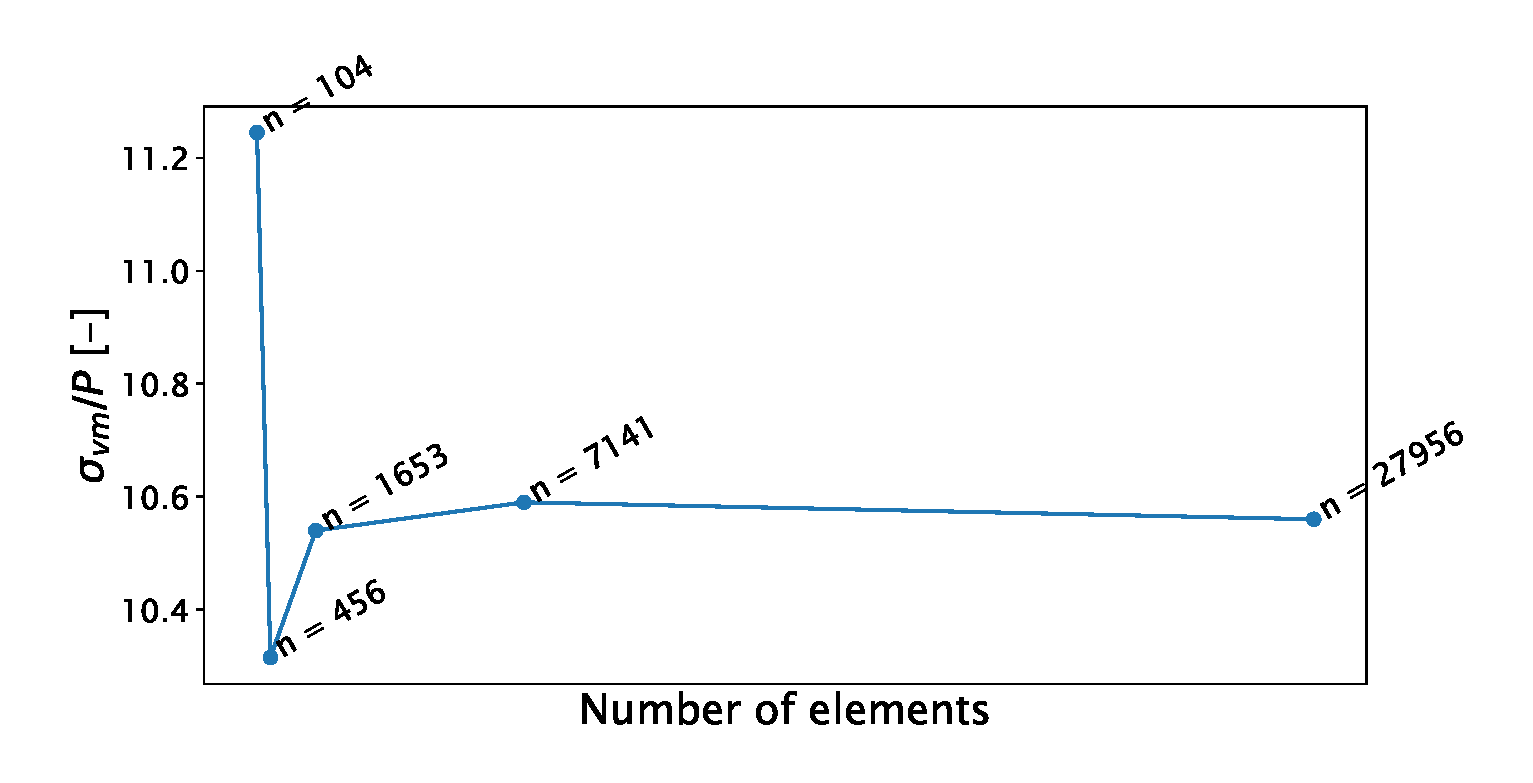
\includegraphics[width = 0.8\textwidth ]{figures/mesh_convergence.eps}
    \caption{Mesh convergence study: Normalized maximum von Mises stress.}
    \label{fig:mesh_convergence}
\end{figure}

\begin{table}[H]
    \centering
    \caption{Numerical model mesh information for the L-shaped bracket.}
    \begin{tabular}{l c c} \hline
        Number of elements ($N$) & Smallest dimension [mm] & Relative error[\%] \\ \hline
        104 & 10.0 & - \\
        456 & 5.000 & 9.02 \\
        1653 & 2.500 & 2.13 \\
        7141 & 1.250 & 0.47 \\
        27956 & 0.625 & 0.28 \\ \hline
    \end{tabular} 
    \label{tab:mesh_convergence}
\end{table}

\begin{figure}[ht]
    \centering
    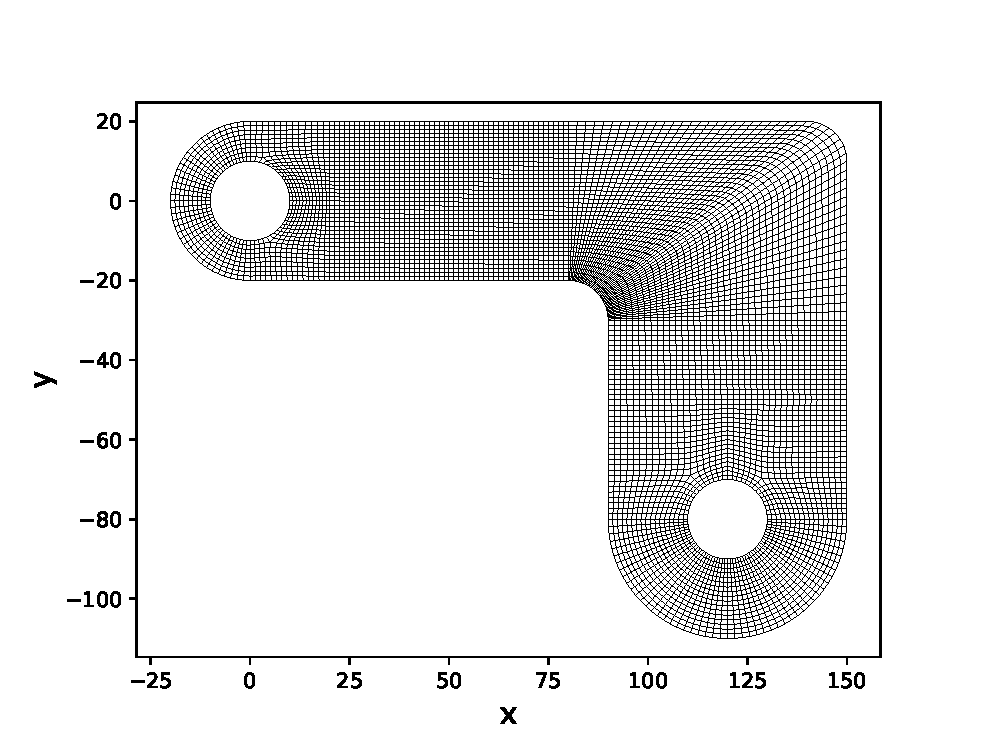
\includegraphics[width = 0.7\textwidth ]{figures/frame_mesh_quality.eps}
    \caption{Mesh quality of the numerical model.}
    \label{fig:mesh_quality}
\end{figure}

\subsection{Element Type}
The quadratic element CPS8R (an 8-node quadratic plane stress element with four integration point) is chosen over the linear CPS4R (a 4-node linear plane stress element with one integration point) (see \cref{fig:element}(a)) as the shape function of the quadratic element is of second-order which suitably characterizes the deformation around curved edges/surfaces. Indeed, the quadratic elements are capable of capturing the geometric features of the deformed state with fewer elements compared with the linear elements (\cref{fig:element}(c)). However, one should know that the quadratic elements are more computationally expensive compared to the linear elements; thus, the proper element type should be chosen accordingly. The suffix $R$ in the name of the element indicates the reduced version of the element (\cref{fig:element}(b)). Due to a refine mesh around the potential areas of concentrated stress, the reduced version suffices. 


\begin{figure}[H]
    \centering
    \includegraphics[width = 0.7\textwidth ]{figures/element.pdf}
    \caption{(a) The full CSP4 and CSP8 element. (b) The CSP4R and CSP8R element. (c) The deformed CSP4 and CSP8 elements. The black dot and cross indicate the node and integration points, respectively.}
    \label{fig:element}
\end{figure}

\subsection{Result and Discussion}
\cref{fig:frame_vm_stress} shows the distribution of the von Mises stress in the L-shaped bracket. As expected, the stress distribution around the support should be critical and gradually relaxes as one moves in the positive $x$-direction. As is seen, the maximum $\sigma_{vm} = 211.8$MPa. Unfortunately, the yield stress of the material is not included; thus, we invoke the value of 250MPa\footnote{Young's Modulus - Tensile and Yield Strength for some common Materials. www.engineeringtoolbox.com/young-modulus-d-417.html. [Online; accessed 08-October-2021]}. Since the von Mises criterion does not violate the assumed yielding stress; therefore, the bracket does not yield. \\

Let us hypothesize about a scenario where the von Mises stress exceeds the yielding stress of the bracket. Let the yielding stress 210MPa then the maximum von Mises is bigger than the yielding stress which contradicts the von Mises concept (which is the maximum value that the von Mises is equal to the yielding stress). The problem arises from the linear elastic analysis. The linear elastic solver computes the displacements at nodes and then extrapolate them to integration points where the strains are calculated. Next, the solver utilizes the linear stress-strain relationship to compute the stresses at the integration points and extrapolates them to nodes. During this process, the solver does not distinguish a yielding point unless specified by the user because the solver follows the linear relation between stress and strain. \\

The displacement magnitude gradient is depicted in \cref{fig:frame_displacement} where the hole under pressure experiences the maximum displacement.

\begin{figure}[ht]
    \centering
        \begin{subfigure}{0.8\textwidth}
            \includegraphics[width=1\linewidth]{figures/frame_vm_stress.png} 
            \caption{}
            \label{fig:frame_vm_stress}
        \end{subfigure}
        
        \begin{subfigure}{0.8\textwidth}
            \includegraphics[width=1\linewidth]{figures/frame_displacement.png} 
            \caption{}
            \label{fig:frame_displacement}
        \end{subfigure}
    \caption{(a)The distribution, minimum and maximum value of von Mises stress (in MPa) (b) The magnitude, minimum and maximum of displacement (in mm) of the L-shaped bracket (Deformation scale factor=1).}
    % \label{fig:}
\end{figure}

%\newpage
%\bibliography{ref}
%\bibliographystyle{ieeetr}

\end{document}